% !TEX root = ../../report.tex

\section{Fashion Recommendation}

%When you enter a clothing store you are normally confronted with the following suggestions:
%    - New in/Seasonal highlights
%    - Special offer/discounts
%    - Bestsellers
%    - Are you looking for something in particular?

\marginpar{heri-notes: hvordan relateres dette til arbeidet deres?}

\subsection{Theory}
  \label{subsec:theory}
  This subsection will look into some background research on fashion.  And look
  into what fashion is and why a consumer behaves like the consumer does.

\subsubsection{What is fashion}
  There are a lot of different ways of defining what fashion really is.

  \begin{itemize}
      \item The entire spectrum of attractive clothes styles at any given time -
      Anne Hollander
      \item Fashion is dress in which the key feature is rapid and continual
      changing of styles - Elisabeth Wilson
      \item Fashion is usually first raised by a small group of people and then a
      trend is formed with more and more followers and copycats till it becomes
      outdated - Cheng \& Huang
      \item The social norm recognized and advocated by a particular social class
      at one time. It affects all the fields in society, especially and famously
      in clothing. Sometimes, short-lived fashion is referred to as style - Fang
      Ma \cite{Fang2012}
  \end{itemize}

  As seen from the different definitions mentioned above, what is reoccurring is;
  clothes, popularity, time and a cultural grouping.
  One of the main drives of fashion is the need and want for belonging, for the individuals to become a part of something bigger and sharing a common though or view.
  So fashion is what a \textbf{social group}, or a \textbf{set of groups}, recognizes and highly advocates \textbf{at any one time}.
  More generally, fashion is a popular style or practice, other categories such as music style and hairstyle can also be viewed as fashion, but in this case the focus will be directed towards clothing.

\subsubsection{Task of fashion marketing}
  Fashion is subject to constant change as seen from the different definitions of
  fashion.

  Some of these changes are due to human changes such as adoption of a new line
  of clothing, or something less controllable, such as the changing of the
  seasons.

  How much of a product should be made to satisfy the need of the consumer, but
  still remain a desirable product the consumer would find itself unique and
  special with?

  What is a reasonable price for the product, and how much is the name of the
  designer worth?  Who can distribute the product without the product loosing its
  value and fashion status?  These are just some of the questions the fashion
  industry has to answer.  Without them answered the potential of the product
  is more difficult to reach.  Which could lead the consumer not to feel the uniqueness and
  prestige of the item.  Fashion trends comes and goes, and the new fashion
  starts with the refusal of what is old.

  In fashion there is a big difference between men and women in what, where, when
  and how they buy.  How to understand the behaviour of the consumers and how they
  act can come from a vast set of areas, the main factors influencing the
  consumer according to \cite{kotler2009marketing} is:

  \begin{table}[H]
      \centering
      \begin{tabular}{l l}
      \toprule
        Factors        			& Examples \\ \midrule
        Physiological factors   & Physical protection, commodity \\
        Socio-cultural factors  & Family, friends, work, social groups  \\
        Personal factors        & Age, life cycle, occupation, personality \\
        Psychological factors   & Product reliance or sympathy \\  % more expensive because more expensive - increase self-confidence
        Rational factors        & Brand of product, quality, designer, price \\
      \bottomrule
      \end{tabular}
      \caption[Fashion Factors]{Main factors influencing the consumer when it comes to their buying behaviour}
      \label{table:FashionFactors}
  \end{table}
  When it comes to fashion it is mainly a socio-cultural phenomenon.

  One central factor when it comes to shopping and fashion is price, a rational factor.
  The consumer acts rational, when it comes to price and quality~\cite{Hanf1994}.
  In the case of fashion, and a product connected with prestige, this rational
  behavior might not apply.

  There is a set of product criteria a consumer evaluates when it comes to the
  acquisition of a product~\cite{dutton2006}, attributes found to have the most
  significant impact is styling, brand , price, place(store), fabrication/fiber
  content.  The complete list is shown in~\ref{table:ConsumersPurchaseDec}


  \marginpar{TODO: Fix some kind of left align centering og content}
  \begin{table}[H]
      \centering
      \begin{tabular}{ccc}
      \toprule
        \multicolumn{2}{c}{Concrete Attributes (Product Features)} & Abstract Attributes (Attitude-Based) \\
        \cmidrule(r{1em}){1-2}
        \multicolumn{1}{c}{Intrinsic (Hedonic)} & \multicolumn{1}{c}{Extrinsic} 				 	& \\ \midrule
        Style 				& Price						 	& Fun \\
        Color				& Brand 					 	& Entertainment \\
        Patten 				& Country of origin			 	& Enjoyment\\
        Fabric/fiber 		& Place(Store) 				 	& Need \\
        Appearance	   	 	& Salespeson's evaluation	 	&  Function\\
        Fashionability  	& Approval of others 		 	&\\
        Durability			& Coordination with wardrobe 	&\\
        Comfort				&								& \\
        Quality				&								& \\
        Fit					&								& \\
        Care 				&								& \\
      \bottomrule
      \end{tabular}
      \caption[Consumers' Purchase Decisions]{The attributes effecting the consumer when in the process of consuming products~\cite{dutton2006}}
      \label{table:ConsumersPurchaseDec}
  \end{table}

  The modern consumer finds pleasure with the consumption experience itself, not
  just the product, and this especially applies to the fashion domain.  The
  purchase is often not done by need, but for pleasure.

  The society nowadays is driven by consumption and change.
  Clothes lets the user claim a position of either respectability or outrageousness, economic and social values~\cite{barnard2002fashion}.
  The clothes of the user is a way of telling the world who the user is.
  Fashion marketing starts and ends at the customer.
  The market must identify the way the consumer dresses himself or herself, and the product has to be produced according to the wants and needs of the user.
  Since this want and need of the user is ever-changing and changing faster and faster, focus must be given to the users actions and want.

  More generally, the fashion marketing must answer the following questions~\cite{vignali2009fashion}:
  \marginpar{These are not really questions?}

  \begin{itemize}
    \item Find consumer needs
    \item The most adequate consumer segment and how to approach
    \item Ideal positioning to reach this segment
    \item Design level, colors, quality that the target segment requires
    \item Price to establish
    \item Channel distribution demands
    \item Marketing strategies and policies that best suit the market segment
  \end{itemize}

  For the market to best answer the customers need, the market must have the best answers to the list above.
  This makes the domain of fashion more difficult to make recommendations for than many other domain, such as movie recommendations and music.

\subsubsection{Consumer buying behavior}
  A lot of information about the consumers behavior is lost due to the reasons
  for their behavior is held in an unconscious or implicit level.  The reason for
  a person is interested in a specific product could be based on some distant
  memory of the consumers life.  This could affect how a consumer views a
  particular brand or product for better or worse.  Brand choices are often made
  intuitively, based on their subconscious, and the consumer cannot tell why
  they made that specific choice~\cite{vignali2009fashion}.

  Culture is one of the main factors to determine consumer behavior.  Culture can
  be segmented into three parts: Culture, subculture and social class.  All
  consumers are included in many smaller subcultures such as nationality,
  religious subcultures and geographical subcultures.  Subcultures can be a
  efficient way of constructing marketing campaigns and aim similar products at,
  since they tend to form market segments.  The forming of a subculture happens
  through individuals seeking out other individuals with similar tastes regarding
  a variety of aspects~\cite{vignali2009fashion}.

  There are a lot of different behavior emerging from subcultures, such as peer
  pressure.  Social psychology is used to understand the behavior of the
  individuals in subcultures~\cite{vignali2009fashion}.

  The brand of the product might also greatly affect what the consumer buys and
  what the consumer does not buy.  A study done on the behavior of the
  consumer~\cite{deLace2010} showed that knowing the brand of two almost
  identical products made the consumer crowd shift towards the more well known
  brand.  Whereas before knowing the actual brand of the product, the crowd had a
  more equal distribution on the products.

\subsubsection{Customer satisfaction}
  There are two main concepts when it comes to customer satisfaction: Transaction
  specific and cumulative specific.  The transaction specific satisfaction of the
  consumer is base on the expectations in the pre-purchase stage and the
  perceived performance of the product in the post-purchase stage.  Where the
  cumulative looks at the purchase as a whole, such as: the product, the purchase
  and the service received~\cite{kumari2012}.  The transaction specific focuses
  on the post-purchase, if the expectations of the product during the
  pre-purchase is met in the post-purchase stage, the likeliness of a repeat
  purchase is increased.

\subsection{Challenges}
  There is a set of challenges when it comes to making recommendations in the
  fashion domain compared to other domains.

\subsubsection{Recentness of items}
  As seen from the different definitions of fashion, time is central in fashion.
  Therefore is time also central when it comes to making recommendations in this
  domain.  What is of interest for the customer one month might not be of
  interest the next.  The interest of the customer is not only affected by what
  is categorized as current fashion, but might be affected by other aspects, such
  as the current season.  The recentness of an item and how long an item is of
  interest for a customer is greatly affected by the customers social groups, and
  the trend in this group.

\subsubsection{How to use user feedback}
  The feedback from the user will mainly be implicit~\ref{sec:implicit}.  As seen
  earlier in this section, it can be assumed that an increased interest in an
  item has some correlation with increased interaction with the item.  To what
  degree this increased interest can be mapped to a more tangible feedback
  varies from customer to customer.
  How the item interaction feedback retrieved will be used is explored in section~\ref{sec:implicit}

  %   - What do we look at? What information is the most useful
  %       - Item category, item keywords, brand... ?
  %   - Changing interest of users

\subsubsection{Product semantics}
  The product database consist of items from multiple stores with multiple
  languages and multiple ways of labeling, describing and categorizing their
  products.  This poses an issue for recommending items based on their content.

  % Building Recommender Systems using a Knowledge Base of product semantics
  % http://images.accenture.ca/SiteCollectionDocuments/PDF/recommenderws02.pdf
  %   - Would probably require some more product semantics...
  %   - Unstructured content/multiple content providers
      % - How to select features for a content-based approach
          % E.g. keywords, when descriptions are in multiple languages
      % - Can rating infromation from similar items be used to decrease sparsity? (Content infromation - Hybrid approaches)

% mtodo: discussion
\marginpar{heri-notes: hvorfor er disse utfordringene relevante for oss?}

\subsection{Fashion in E-commerce}
  \label{subsubs:fashionInEcom}
  E-commerce is usually known as trading services and products via the Internet. There are many different services and products traded, such as fashion products. Fashion is one of the sectors in e-commerce increasing the most in many countries. In UK the online fashion sector has grown 258\% in five years~\cite{Divante2014}. Three months after GANT~\cite{gant} launched their new e-commerce solution, their orders online increased by 340\%~\cite{magentoGant}.

  Previous sections has mentioned that a consumer is consuming for the satisfaction of consumption, which might not completely agree with the GANT example, but numbers from Statistics Norway~\cite{statisticsNorway} shows that fashion e-commerce is increasing at a high rate.

  \begin{figure}[H]
    \centering
    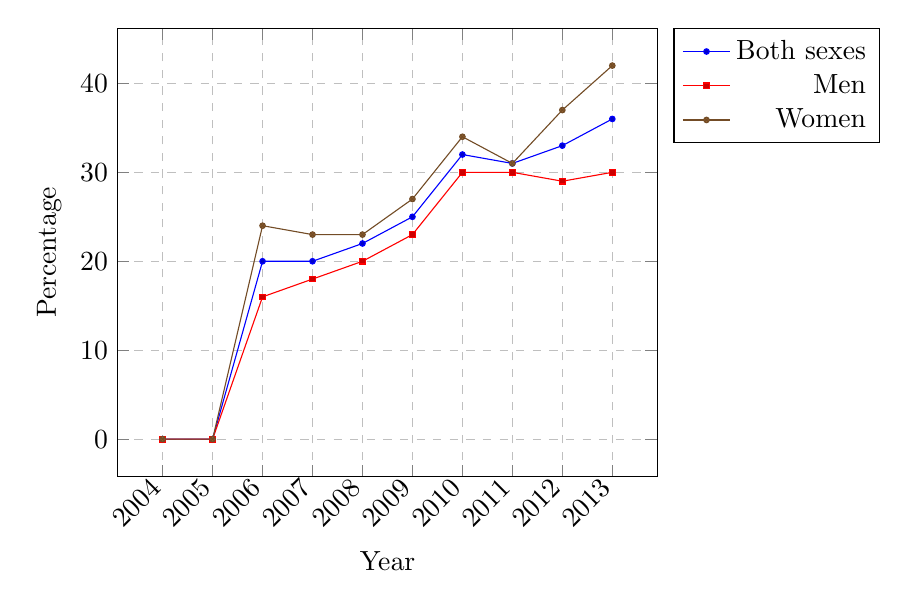
\begin{tikzpicture}
      \begin{axis}[
        xlabel={Year},
        ylabel={Percentage},
        legend style={cells={anchor=east}, legend pos=outer north east,},
        xtick=data,
        x tick label style={rotate=45, anchor=east, /pgf/number format/1000 sep=},
        mark size=1.0pt,
        grid=major,
        grid style={dashed},
      ]
      \legend{Both sexes, Men, Women, Regression}
      \addplot coordinates {
        (2004, 0)
        (2005, 0)
        (2006, 20)
        (2007, 20)
        (2008, 22)
        (2009, 25)
        (2010, 32)
        (2011, 31)
        (2012, 33)
        (2013, 36)
      };
      \addplot coordinates {
        (2004, 0)
        (2005, 0)
        (2006, 16)
        (2007, 18)
        (2008, 20)
        (2009, 23)
        (2010, 30)
        (2011, 30)
        (2012, 29)
        (2013, 30)
      };
      \addplot coordinates {
        (2004, 0)
        (2005, 0)
        (2006, 24)
        (2007, 23)
        (2008, 23)
        (2009, 27)
        (2010, 34)
        (2011, 31)
        (2012, 37)
        (2013, 42)
      };
      \end{axis}
    \end{tikzpicture}

    \caption[Statistics of e-commerce purchase in Norway]{This figure is taken
    from~\cite{statisticsNorway} and shows the growth of online purchases through
    e-commerce applications in Norway}
  \end{figure}


  \begin{figure}[H]
      \centering
      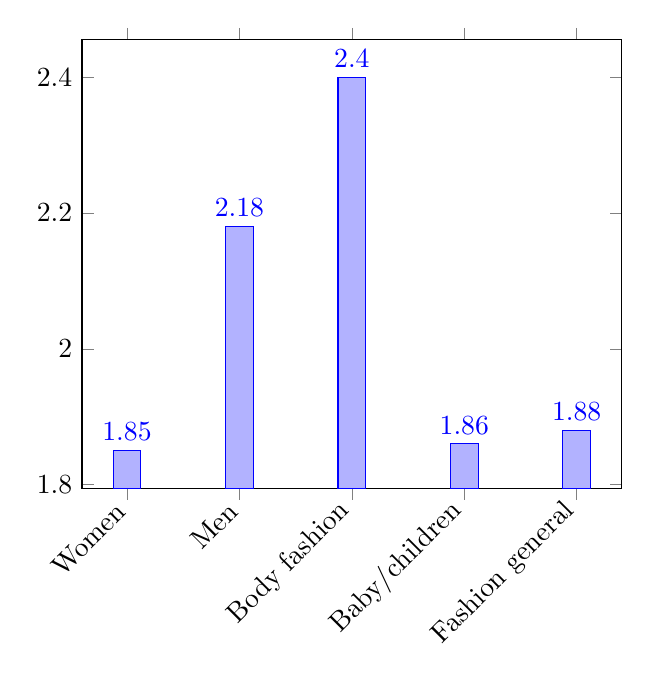
\begin{tikzpicture}
        \begin{axis}[
          ybar,
          symbolic x coords={Women, Men, Body fashion, Baby/children, Fashion general},
          x tick label style={rotate=45, anchor=east},
        ]
        \addplot +[nodes near coords] coordinates {
          (Women, 1.85)
          (Men, 2.18)
          (Body fashion, 2.40)
          (Baby/children, 1.86)
          (Fashion general, 1.88)
        };
        \end{axis}
      \end{tikzpicture}

      \caption[Conversion Rate in Fashion Retail]{This figure is taken from~\cite{Jorij2012} and shows the different values for conversion rate in the fashion domain.
      Conversion rate is the portion of users who visits a website, who goes beyond only browsing items and reaches some goal achievements.
      These goal achievements can be actions such as product purchase or advertisement interaction.
      The conversion rate is then $Conversion rate = \frac{\# of Goal Achievments}{Visits}$~\cite{nielsen2013}.
      As seen from this figure, womens fashion has the lowest conversion rate in the different types of e-commerce fashion.
      The average conversion rate in e-commerce was around 3\% in 2013~\cite{nielsen2013}.
      }
  \end{figure}

  \begin{figure}[H]
    \centering
    \begin{tikzpicture}
      \pie[text=legend, rotate=60]{
        34.30/Women,
        13.43/Men,
        17.91/Generalist,
        11.94/Body,
        4.47/Shoes,
        2.98/Jeans,
        14.97/Other
      }
    \end{tikzpicture}
    \caption[E-commerce benchmark and Fashion]{This figure is taken from~\cite{Jorij2012} and shows how the different e-commerce fashion retailers focuses their products.
    This figure is based on 70 different fashion companies.
    It is clear that the large portion of the e-commerce fashion companies are putting their focus on women's clothing.}
  \end{figure}

  \begin{figure}[H]
    \centering
    \begin{tikzpicture}
      \pie[text=legend, rotate=60]{
        15/Direct,
        23/Paid,
        30/Organic,
        5/CPS,
        9/CPC,
        8/Viral or social,
        10/E-mail newsletter
      }
    \end{tikzpicture}
    \caption[Traffic Sources In Fashion]{This figure is taken from~\cite{Jorij2012} and shows where the users originated from in e-commerce fashion.
    Paid and Organic are search engine origins, and is 53\% of traffic origin in e-commerce fashion.
    Direct traffic is at 15\%, the average direct hit in e-commerce application is 22.3\%.
    \cite{Jorij2012} explains this with the fact that the same products are often available on multiple e-commerce web sites, and the user browses for the best offer.
    Even though the viral/social origin segment is rather small (8\%) the average for e-commerce companies is 4\%.
    The social media is much more influential on e-commerce companies regarding fashion than other e-commerce companies.}
  \end{figure}

\subsection{SoBazaar, the e-commerce application}
  As briefly mentioned in the introduction chapter~\ref{sec:motivation} SoBazaar is a fashion e-commerce application for web and hand held devices.
  The application is developed by Telenor and aggregates fashion products from various brands and stores, mainly fashion related.
  Users of the application can choose to log in with their social media account on Facebook~\footnote{Facebook is an online social media service with around 1.28 billion monthly active users~\cite{facebook}} to store and share their fashion findings in the application.
  This allows the user to have one entry point to get the latest updates on fashion, and see what the user's social network is up in regards to fashion.
  When the user finds an item especially interesting and is interested in purchasing the item, the user is redirected to the store from which the product originated.

  The fact that SoBazaar utilizes Facebook and a large set of fashion stores lets the users of the application gather at one place to find users with similar taste in fashion.
  As seen from~\ref{subsec:theory} one important aspect in fashion is the feeling of belonging, which is made easy through the utilization of Facebook.

\subsection{Competitors to SoBazaar}

	\marginpar{TODO: Extend with Asos}
	\marginpar{TODO: Extend with Kwoller}
	\marginpar{TODO: Extend with Mallzee}
	\marginpar{TODO: Mention that many new apps have popped up recently, attempting to do the same as SoBazaar}

    As seen from~\ref{subsubs:fashionInEcom} SoBazaar is not the only e-commerce application for fashion, and has therefore some competitors.
    SoBazaar is built up of a collection of e-commerce store front applications and social interactions, but SoBazaar is not the first of its kind.
    There is a set of other similar applications providing the user with similar possibilities as SoBazaar.
    This section will be used to explore some of these systems, and look into their strengths and weaknesses regarding item recommendation for the user.

\subsubsection{Myntra} % (fold)
\label{par:myntra}
    "Myntra.com is a one stop shop for all your fashion and lifestyle needs" - about Myntra~\cite{myntra}.

    Myntra is one of India's largest e-commerce stores for fashion and aims to  provide a hassle free shopping experience for the user.
    They aim to bring the newest and most in-season fashion products available to the user trough the web store front.
    The brand base of Myntra consists of 500 leading brands from both inside and outside India.

    The web page uses a set of recommendation approaches to inform the user of what they might like, and to increase the user's awareness of different kinds of items. Such as, similar item and most popular.

    \begin{figure}[H]
        \centering
        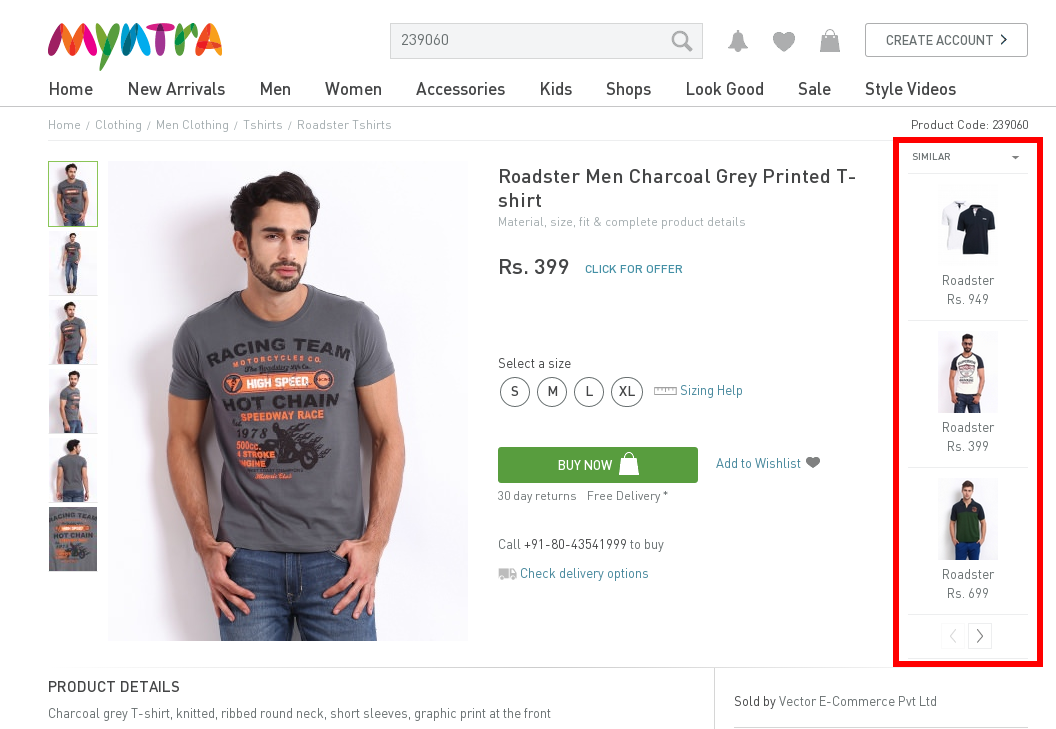
\includegraphics[width=5in]{image/myntiaSimilarExample.png}
        \caption[Example of Myntra's "similar item" approach]{In this figure we can see in red how Myntra is suggesting items which are similar to the item the user is currently looking at}
        \label{figure:myntiaSimilarEx}
    \end{figure}

    \begin{table}[H]
        \centering
        \begin{tabularx}{\linewidth}{>{\parskip1ex}X@{\kern4\tabcolsep}>{\parskip1ex}X}
            \toprule
            \hfil\bfseries Strengths
            &
            \hfil\bfseries Weaknesses
            \\\cmidrule(r{3\tabcolsep}){1-1}\cmidrule(l{-\tabcolsep}){2-2}
            %Strengths
	        Suggest similar items connected to the currently viewed \par
            Popular list for the different brands and stores \par
            Ability to add item to a "want list"\par
            &
            %Weaknesses
            No personalized recommendations \par
            \\\bottomrule
        \end{tabularx}
        \caption[Recommendation related strengths and weaknesses of Myntra~\cite{myntra}]{This table is the list of the recommendation related strengths and weaknesses of the e-commerce fashion web site Myntra~\cite{myntra}}
        \label{table:ecommerceMyntra}
    \end{table}
% paragraph myntra (end)

\subsubsection{Flink} % (fold)
\label{par:flink}
    "Flink is THE brand-new app to discover, get inspired and share trendy looks from top fashion bloggers" - About Flink~\cite{flink}.

    Flink is a fashion discovery application for iPhone.
    It allows the user to browse fashion blogs, hot brands and new trends.

    The content displayed can be "liked" and can be a collection of clothes from different brands.
    If the user is interested in the item, the application can redirect the user to the web page where it is sold.
    \begin{table}[H]
            \centering
            \begin{tabularx}{\linewidth}{>{\parskip1ex}X@{\kern4\tabcolsep}>{\parskip1ex}X}
                \toprule
                \hfil\bfseries Strengths
                &
                \hfil\bfseries Weaknesses
                \\\cmidrule(r{3\tabcolsep}){1-1}\cmidrule(l{-\tabcolsep}){2-2}
                Can follow other users \par
                Connect with facebook \par
                Ability to add item to a \emph{want list} \par
                &
                No personalized recommendations \par
                \\\bottomrule
                \end{tabularx}
        \caption[Recommendation related strengths and weaknesses of Flink~\cite{flink}]{This table is the list of the recommendation related strengths and weaknesses of the mobile fashion application Flink~\cite{flink}}
        \label{table:iphoneAppFlink}
    \end{table}
  % todo - might be more, but can't explore the application since it is iOS 7 required
% paragraph flink (end)

\subsubsection{Lyst} % (fold)
\label{par:lyst}
    "Lyst.com is a fashion shopping site that gives you your own shopping experience, so you can discover more of the fashion you love" - About Lyst~\cite{lyst}.

    Lyst offers items from thousands of the leading brands and stores of the world.

    The site allows the user to follow different stores or brands to receive the latest items they have to offer.
    The user is given a personalized "stylefeed", which displays items from the different brands or stores the user is following.
    It is also possible for the user to add items to the their profile.

    On first login the user is presented with a set of brands and store the user can like or dislike, to get the "stylefeed" started.
    On access of an item, the user is presented with related items, and the ability to add the item to a collection.
    When the user wants to buy an item, the site will redirect the user to the store selling the item.

    \begin{table}[H]
    	\centering
        \begin{tabularx}{\linewidth}{>{\parskip1ex}X@{\kern4\tabcolsep}>{\parskip1ex}X}
        \toprule
        	\hfil\bfseries Strengths
            &
            \hfil\bfseries Weaknesses
            \\\cmidrule(r{3\tabcolsep}){1-1}\cmidrule(l{-\tabcolsep}){2-2}
                    Can follow brands and stores \par
                    Connected with facebook \par
                    Ability to add item to a "want list" \par
                    "Stylfeed" based the user's follow list \par
                    Show related items \par
                    &
                    Limited personalized recommendations \par
                    \\\bottomrule
                \end{tabularx}
        \caption[Recommendation related strengths and weaknesses of Lyst~\cite{lyst}]{This table is the list of the recommendation related strengths and weaknesses of e-commerce fashion web site Lyst~\cite{lyst}}
        \label{table:ecommenreceLyst}
    \end{table}
% paragraph lyst (end)

\subsubsection{Motilo} % (fold)
\label{par:motilo}
    "Motilo was launched in 2011 to answer that perennial fashion dilemma all women face – what shall I wear tonight?" - About Motilo~\cite{motilo}.

    Items on the web page are gathered by the Motilo stylists.
    This gives the page a fresh set of items for the user to select from.

    Motilo gives the user the ability to put together item sets through dragging and dropping the items into a "fashion dilemma", or simply like items.
    The user can ask friends, the Motilo community or the Motilo stylists about suggestions regarding what to wear.
    If the user wants to buy an item, Motilo redirects the user to the page which sells the item in question.

    \begin{table}[H]
    \centering
    \begin{tabularx}{\linewidth}{>{\parskip1ex}X@{\kern4\tabcolsep}>{\parskip1ex}X}
    	\toprule
    	\hfil\bfseries Strengths
    	&
    	\hfil\bfseries Weaknesses
    		\\\cmidrule(r{3\tabcolsep}){1-1}\cmidrule(l{-\tabcolsep}){2-2}
            Connected with facebook \par
            Ability to add item to a "want list" \par
            A feed with the most trending item collections \par
            Ask Motilo stylists for suggestions \par
            &
            Manual/limited personalized recommendations \par
            \\\bottomrule
            \end{tabularx}
            \caption[Recommendation related strengths and weaknesses of Motilo~\cite{motilo}]{This table is the list of the recommendation related strengths and weaknesses of e-commerce fashion web site Motilo~\cite{motilo}}
            \label{table:ecommenreceMotilo}
        \end{table}


% paragraph motilo (end)


\subsubsection{Farfetch} % (fold)
\label{par:farfetch}
    "farfetch.com forms the hub of a global fashion community that unites independent boutiques around the world with fashion lovers" - About Farfetch~\cite{Farfetch}

    Farfetch is a collection of over 1000 boutiques from all over the world gathered on one web page.
    The user can shop directly on the page, and get the item delivered to the doorstep with only one checkout process.

    When browsing an item the user is presented with a set of recommendations related to the current item, and previous browsing history.
    The item can be added to a "want list" or to the shopping chart.
    \begin{figure}[H]
        \centering
        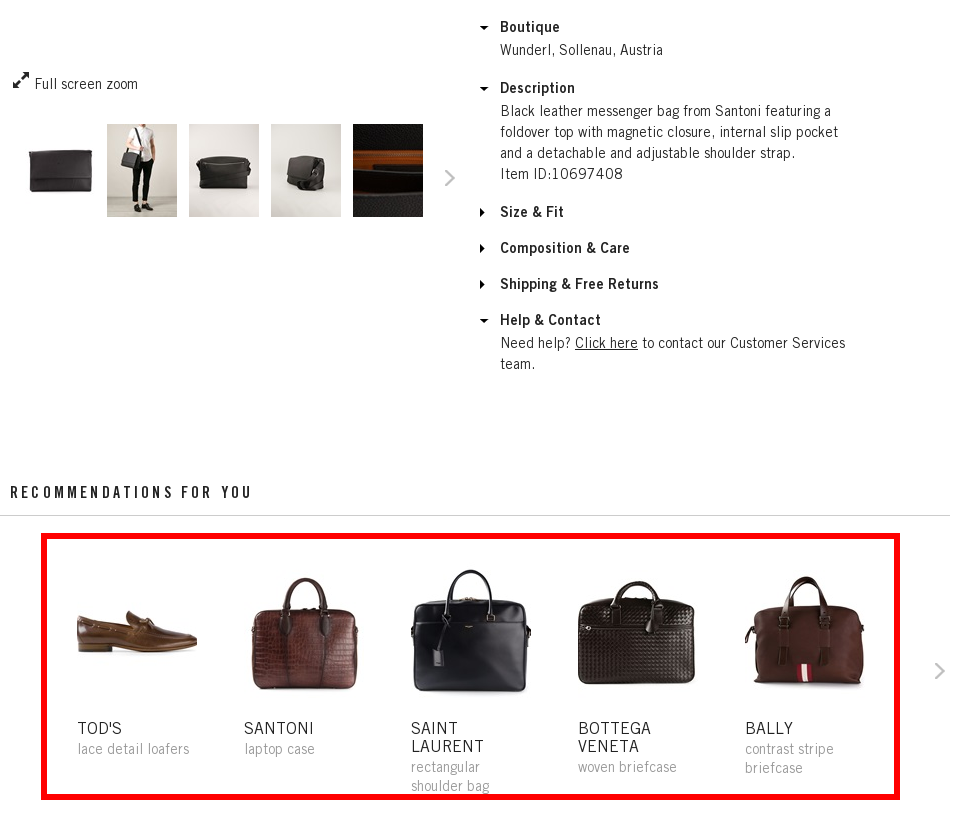
\includegraphics[width=5in]{image/farfetchedRecommendationExample.png}
        \caption[Example of Farfetch's recommendations]{In this figure we can see in red how Farfetch is recommending items which might be of interest to the user. As we can see the first item is a shoe, which was the last item accessed by the user, the next four items are related to the currently viewed item}
        \label{figure:farfetchedRecommendationExample}
    \end{figure}
    \begin{table}[H]
        \centering
        \begin{tabularx}{\linewidth}{>{\parskip1ex}X@{\kern4\tabcolsep}>{\parskip1ex}X}
        	\toprule
        	\hfil\bfseries Strengths
        	&
        	\hfil\bfseries Weaknesses
        		\\\cmidrule(r{3\tabcolsep}){1-1}\cmidrule(l{-\tabcolsep}){2-2}
        		%Strengths
                Ability to add item to a "want list" \par
                A feed with the most popular items \par
                A feed with new items \par
                A list of recommendations for the user \par
            	&
            	%Weaknesses
                No option to follow other users \par
             \\\bottomrule
        \end{tabularx}
        \caption[Recommendation related strengths and weaknesses of Farfetch~\cite{Farfetch}]{This table is the list of the recommendation related strengths and weaknesses of e-commerce fashion web site Farfetch~\cite{Farfetch}}
        \label{table:ecommenreceFarfetch}
    \end{table}
% paragraph farfetch (end)


\subsubsection{ModCloth} % (fold)
\label{par:modcloth}
    "A top e-retailer of indie clothing, accessories, and decor, and provide an engaging shopping experience where you, our customer, can have a voice" - About ModCloth~\cite{modcloth}

    ModCloth focuses on giving what the community is looking for.
    The user is given the opportunity to both be the seller and the buyer.
    The item base is affected by the user trough voting.
    \begin{table}[H]
            \centering
            \begin{tabularx}{\linewidth}{>{\parskip1ex}X@{\kern4\tabcolsep}>{\parskip1ex}X}
            	\toprule
            	\hfil\bfseries Strengths
            	&
            	\hfil\bfseries Weaknesses
            	\\\cmidrule(r{3\tabcolsep}){1-1}\cmidrule(l{-\tabcolsep}){2-2}
                Ability to add item to a "want list" \par
                A feed with the most popular items \par
                A feed with new items \par
                A list of similar items \par
            	&
                No personalized recommendations \par
            	\\ \bottomrule
        \end{tabularx}
        \caption[Recommendation related strengths and weaknesses of
        ModCloth~\cite{modcloth}]{This table is the list of the recommendation
        related strengths and weaknesses of e-commerce fashion web site
        ModCloth~\cite{modcloth}}
        \label{table:ecommenreceModCloth}
    \end{table}
% paragraph modcloth (end)


\subsubsection{UsTrendy} % (fold)
\label{par:ustrendy}
    "UsTrendy allows you to shop and discover one-of-a-kind fashions from all over the world." - About UsTrendy~\cite{UsTrendy}

    UsTrendy has a large item database of more than hundred thousand unique items.

    When the user is viewing an item, UsTrendy displays other items the user might like, which have common traits with the one the user is currently watching.
    The currently viewed item can be added to a sopping cart.
    \begin{table}[H]
                \centering
                \begin{tabularx}{\linewidth}{>{\parskip1ex}X@{\kern4\tabcolsep}>{\parskip1ex}X}
                	\toprule
                	\hfil\bfseries Strengths
                	&
                	\hfil\bfseries Weaknesses
                	\\\cmidrule(r{3\tabcolsep}){1-1}\cmidrule(l{-\tabcolsep}){2-2}
                  Ability to add item to a "want list" \par
                  A feed with the most popular items \par
                  A feed with new items \par
                  A list of similar items \par
             	  &
                  No personalized recommendations \par
                \\ \bottomrule
        \end{tabularx}
        \caption[Recommendation related strengths and weaknesses of UsTrendy~\cite{UsTrendy}]{This table is the list of the recommendation related strengths and weaknesses of e-commerce fashion web site UsTrendy~\cite{UsTrendy}}
        \label{table:ecommenreceUsTrendy}
    \end{table}
% paragraph ustrendy (end)


\subsubsection{Polyvore} % (fold)
\label{par:polyvore}
    "Polyvore is a new way to discover and shop for things you love." - About Polyvore~\cite{polyvore}

    In Polyvore the user can put together sets of items and show them off to their friends and others.
    The items shown on Polyvore are gathered based on the community of Polyvore.

    When accessing an item the user is shown similar items to the one which is currently being watched.
    When the user want to purchase an item, the user is redirected to the page which sells the item.
    \begin{table}[H]
                \centering
                \begin{tabularx}{\linewidth}{>{\parskip1ex}X@{\kern4\tabcolsep}>{\parskip1ex}X}
                \toprule
                \hfil\bfseries Strengths
                &
                \hfil\bfseries Weaknesses
                \\\cmidrule(r{3\tabcolsep}){1-1}\cmidrule(l{-\tabcolsep}){2-2}
                	Ability to add item to a "want list" \par
                	The user can follow other users \par
                	Crawl other fashion sites to add to their item base \par
                	A feed with trending items \par
                	A list of recently viewed items \par
            	&
                	No personalized recommendations \par
                \\ \bottomrule
        \end{tabularx}
        \caption[Recommendation related strengths and weaknesses of
        Polyvore~\cite{polyvore}]{This table is the list of the recommendation
        related strengths and weaknesses of e-commerce fashion web site
        Polyvore~\cite{polyvore}}
        \label{table:ecommenrecePolyvore}
    \end{table}
% paragraph polyvore (end)


\subsubsection{Clothia} % (fold)
\label{par:clothia}
    "An online destination where you can mix and match outfits, share looks you love, even try on clothes virtually via your webcam using augmented reality technology" - About Clothia~\cite{clothia}

    The user can put together a set of clothes from the web site and make a "set".
    The set can be shared with other users and like by other users.
    If the user is interested in buying an item, the user is redirected to the page from which the item is sold.
    \begin{table}[H]
                \centering
                \begin{tabularx}{\linewidth}{>{\parskip1ex}X@{\kern4\tabcolsep}>{\parskip1ex}X}
                \toprule
                \hfil\bfseries Strengths
                &
                \hfil\bfseries Weaknesses
                \\\cmidrule(r{3\tabcolsep}){1-1}\cmidrule(l{-\tabcolsep}){2-2}
                Ability to add item to a "want list" \par
                The user can follow other users \par
                A feed with trending items \par
            	&
                Lack personalized recommendations \par
                \\ \bottomrule
        \end{tabularx}
        \caption[Recommendation related strengths and weaknesses of Clothia~\cite{clothia}]{This table is the list of the recommendation related strengths and weaknesses of e-commerce fashion web site Clothia~\cite{clothia}}
        \label{table:ecommenreceClothia}
    \end{table}
% paragraph clothia (end)


\subsubsection{Trendabl} % (fold)
\label{par:trendabl}
    "Trendabl is a community of people who love fashion" - About Trendable~\cite{trendabl}

    The user is shown a feed with the newest items, and is free to browse different sets of collections, such as collections with shoes and pants.
    If the user wants to buy an item it can be added to a shopping chart.
    \begin{table}[H]
                    \centering
                    \begin{tabularx}{\linewidth}{>{\parskip1ex}X@{\kern4\tabcolsep}>{\parskip1ex}X}
                    \toprule
                    \hfil\bfseries Strengths
                    &
                    \hfil\bfseries Weaknesses
                    \\\cmidrule(r{3\tabcolsep}){1-1}\cmidrule(l{-\tabcolsep}){2-2}
                	Ability to add item to a "want list" \par
	                The user can follow other users \par
                	System recommends the top users in the system for the user to follow \par
            		&
                	No personalized recommendations \par
            		\\ \bottomrule
        \end{tabularx}
        \caption[Recommendation related strengths and weaknesses of Trendabl~\cite{trendabl}]{This table is the list of the recommendation related strengths and weaknesses of e-commerce fashion web site Trendabl~\cite{trendabl}}
        \label{table:ecommenreceTrendabl}
    \end{table}
% paragraph trendabl (end)

\subsubsection{Rue La La} % (fold)
\label{par:rue_la_la}
    "Rue La La is the destination for the most desired brands" - About Rue La La~\cite{RueLaLa}

    Rue La La is a sale on site e-commerce web site.
    It is built up of a set of different boutiques, which can be browsed by the user.
    When the user is watching an item, Rue La La shows other items from the current boutique.

    \begin{table}[H]
                \centering
                \begin{tabularx}{\linewidth}{>{\parskip1ex}X@{\kern4\tabcolsep}>{\parskip1ex}X}
                \toprule
                \hfil\bfseries Strengths
                &
                \hfil\bfseries Weaknesses
                \\\cmidrule(r{3\tabcolsep}){1-1}\cmidrule(l{-\tabcolsep}){2-2}
                Ability to add item to a "want list" \par
                List of most popular items \par
           		&
                No personalized recommendations \par
            	\\ \bottomrule
        \end{tabularx}
        \caption[Recommendation related strengths and weaknesses of Rue La La~\cite{RueLaLa}]{This table is the list of the recommendation related strengths and weaknesses of e-commerce fashion web site Rue La La~\cite{RueLaLa}}
        \label{table:ecommenreceRueLaLa}
    \end{table}
% paragraph rue_la_la (end)

\subsubsection{Zalando} % (fold)
\label{par:zalando}
    "Clothes, accessories, sports items, beauty products" - About Zalando~\cite{Zalando}

    Zalando has a large set of items.
    When browsing an item the user is shown a set of similar items the user might also like, and a set of items which might "go well"  with the currently viewed item.

    \begin{table}[H]
                    \centering
                    \begin{tabularx}{\linewidth}{>{\parskip1ex}X@{\kern4\tabcolsep}>{\parskip1ex}X}
                    \toprule
                    \hfil\bfseries Strengths
                    &
                    \hfil\bfseries Weaknesses
                    \\\cmidrule(r{3\tabcolsep}){1-1}\cmidrule(l{-\tabcolsep}){2-2}
                	Ability to add item to a "want list" \par
                    Shop on site \par
                	Similar items \par
            		&
                	No personalized recommendations \par
             		\\ \bottomrule
        \end{tabularx}
        \caption[Recommendation related strengths and weaknesses of Zalando~\cite{Zalando}]{This table is the list of the recommendation related strengths and weaknesses of e-commerce fashion web site Zalando~\cite{Zalando}}
        \label{table:ecommenreceZalando}
    \end{table}
% paragraph zalando (end)

\subsubsection{Ellos~\cite{Ellos}} % (fold)
\label{par:ellos}
    Ellos is a e-commerce web site, which specializes in fashion.

    When browsing an item, similar items to the one currently being watched is presented to the user.
    Other items which might go well with the item is also presented for the user.

    \begin{table}[H]
                \centering
                \begin{tabularx}{\linewidth}{>{\parskip1ex}X@{\kern4\tabcolsep}>{\parskip1ex}X}
                \toprule
                \hfil\bfseries Strengths
                &
                \hfil\bfseries Weaknesses
                \\\cmidrule(r{3\tabcolsep}){1-1}\cmidrule(l{-\tabcolsep}){2-2}
                Ability to add item to a "want list" \par
                Shop on site \par
                Similar items \par
                On site most popular list \par
                Items which might go well with the current \par
            	&
                No personalized recommendations \par
             	\\ \bottomrule
        \end{tabularx}
        \caption[Recommendation related strengths and weaknesses of Ellos~\cite{Ellos}]{This table is the list of the recommendation related strengths and weaknesses of e-commerce fashion web site Ellos~\cite{Ellos}}
        \label{table:ecommenreceEllos}
    \end{table}
% paragraph ellos (end)

\subsubsection{LookBook} % (fold)
\label{par:lookbook}
    "LOOKBOOK is the \#1 source for fashion inspiration from real people around the world." - About LookBook~\cite{LookBook}

    LookBook is a leading online community which is centered around the looks of the users.
    The users can share their own looks and keep up with other users through watching their uploads.
    With over 1.2 million members LookBook is constantly up to date on the newest fashion trends.
    \begin{table}[H]
                \centering
                \begin{tabularx}{\linewidth}{>{\parskip1ex}X@{\kern4\tabcolsep}>{\parskip1ex}X}
                \toprule
                \hfil\bfseries Strengths
                &
                \hfil\bfseries Weaknesses
                \\\cmidrule(r{3\tabcolsep}){1-1}\cmidrule(l{-\tabcolsep}){2-2}
                Ability to add item to a "want list" \par
                Shop on site \par
                Similar items \par
                Most popular items list \par
                Hot items list \par
             	&
                No personalized recommendations \par
             	\\ \bottomrule
        \end{tabularx}
        \caption[Recommendation related strengths and weaknesses of LookBook~\cite{LookBook}]{This table is the list of the recommendation related strengths and weaknesses of e-commerce fashion web site LookBook~\cite{LookBook}}
        \label{table:ecommenreceLookBook}
    \end{table}
% paragraph lookbook (end)

\subsubsection{Fashiolista} % (fold)
\label{par:fashiolista}
    "Let Fashiolista's community be your style guide in the online fashion jungle" - About Fasho~\cite{Fashiolista}

    The items on Fashiolista is selected by the users of Fashiolista, and the sites is therefore customized to fit the user crowd's wishes and interests.

    When accessing an item, the user is presented with the item, and a set of other items from the store the current item originated from.
    Other users who liked the item are also shown, so the user can browse their personal want list.
    \begin{table}[H]
                    \centering
                    \begin{tabularx}{\linewidth}{>{\parskip1ex}X@{\kern4\tabcolsep}>{\parskip1ex}X}
                    \toprule
                    \hfil\bfseries Strengths
                    &
                    \hfil\bfseries Weaknesses
                    \\\cmidrule(r{3\tabcolsep}){1-1}\cmidrule(l{-\tabcolsep}){2-2}
                Ability to add item to a "want list" \par
                On site most popular list \par
             &
                 No personalized recommendations \par
             \\ \bottomrule
        \end{tabularx}
        \caption[Recommendation related strengths and weaknesses of Fashiolista~\cite{Fashiolista}]{This table is the list of the recommendation related strengths and weaknesses of e-commerce fashion web site Fashiolista~\cite{Fashiolista}}
        \label{table:ecommenreceFahiolista}
    \end{table}
% paragraph fashiolista (end)

\subsubsection{ShopStyle} % (fold)
\label{par:shopstyle}
    "POPSUGAR is a global women's lifestyle brand focused in media, commerce, and technology" - About ShopStyle~\cite{ShopStyle}

    ShopStyle is a commerce brand of POPSUGAR.
    ShopStyle displays items from other e-commerce web sites, and redirects the user directly to the e-commerce web site from which the item clicked originated.
    Items can be liked on ShopStyle, and viewed in less detail at the web page of ShopStyle.
    \begin{table}[H]
                    \centering
                    \begin{tabularx}{\linewidth}{>{\parskip1ex}X@{\kern4\tabcolsep}>{\parskip1ex}X}
                    \toprule
                    \hfil\bfseries Strengths
                    &
                    \hfil\bfseries Weaknesses
                    \\\cmidrule(r{3\tabcolsep}){1-1}\cmidrule(l{-\tabcolsep}){2-2}
                Ability to add item to a "want list" \par
                Similar items \par
                Editor's picks \par
            &
                No personalized recommendations \par
            \\ \bottomrule
        \end{tabularx}
        \caption[Recommendation related strengths and weaknesses of ShopStyle~\cite{ShopStyle}]{This table is the list of the recommendation related strengths and weaknesses of e-commerce fashion web site ShopStyle~\cite{ShopStyle}}
        \label{table:ecommenreceShopStyle}
    \end{table}
% paragraph shopstyle (end)

\subsubsection{MyHabit} % (fold)
\label{par:myhabit}
    "MyHabit is a private fashion sale site offering up to 60% off hand-picked selections from designer and boutique brands." - About MyHabit~\cite{MyHabit}

    MyHabit was founded by Amazon in response to the desire from the users of Amazon to shop fashion in an easy manner.

    The site displays a feed.
    This feed is fed by a team from MyHabit, and is constantly updating with new sales and new products.
    The items put into the feed are handpicked.

    When browsing items on MyHabit, other similar items are suggested to the user.
    \begin{table}[H]
                    \centering
                    \begin{tabularx}{\linewidth}{>{\parskip1ex}X@{\kern4\tabcolsep}>{\parskip1ex}X}
                    \toprule
                    \hfil\bfseries Strengths
                    &
                    \hfil\bfseries Weaknesses
                    \\\cmidrule(r{3\tabcolsep}){1-1}\cmidrule(l{-\tabcolsep}){2-2}
                Shop on site \par
                Similar items \par
             &
                No personalized recommendations \par
            \\ \bottomrule
        \end{tabularx}
        \caption[Recommendation related strengths and weaknesses of MyHabit~\cite{MyHabit}]{This table is the list of the recommendation related strengths and weaknesses of e-commerce fashion web site MyHabit~\cite{MyHabit}}
        \label{table:ecommenreceMyHabit}
    \end{table}
% paragraph myhabit (end)

\subsubsection{Competitors Recommendation Overview} % (fold)
\label{par:competitors_recommendation_overview}
    In table~\ref{table:ecommerceCommpetiros} we see that there is a very low count of fashion related e-commerce applications, which actually produces personalized recommendations for their users.

    Most of applications are taking a simpler approach when making recommendations for the user, like most popular or similar items.
    There is no obvious relation between recommendations and that the site has a form of "want list", but the system which allows the users to follow each other are usually not in-application-purchase-applications.

    There where no indications of the "want list" being used directly to some personalized recommendations and neither was it any indication that the "follow list" of other users helped produce any personalized recommendations, other than recommending items from the followed user's feed.
    The "follow list" was also in some cases used to suggest other users to follow.
    The "want list" was primarily there so that the user could go back to a liked item, and maybe interact with it later.
    \begin{table}[H]
        \centering
        \begin{tabular}{l l l l l l l}
            \toprule
            Competitor &
            \multicolumn{1}{l}{\parbox{1.3cm}{ In App \\ Purchase}} &
            \multicolumn{1}{l}{\parbox{1.0cm}{ Most \\ Popular}} &
            \multicolumn{1}{l}{\parbox{1.0cm}{ Similar \\ Items}} &
            \multicolumn{1}{l}{\parbox{1.0cm}{ Want \\ List}} &
            \multicolumn{1}{l}{\parbox{1.9cm}{ Follow \\ Other Users}} &
            \multicolumn{1}{l}{\parbox{2.6cm}{ Personalized \\ Recommendations}} \\ \midrule

            Myntra  & \cmark & \cmark & \cmark & \cmark & \xmark & \xmark \\
            Flink   & \xmark & \cmark & ?? & \cmark & \cmark & \xmark \\
            Lyst    & \xmark & \cmark & \cmark & \cmark & \cmark & \xmark \\
            Motilo  & \xmark & \cmark & \xmark & \cmark & \cmark & \xmark \\
            Farfetch & \cmark & \cmark & \cmark & \cmark & \xmark & \xmark/\cmark~\tablefootnote{How the recommendations are produced is not mentioned} \\
            ModCloth  & \cmark & \cmark & \cmark & \cmark & \xmark & \xmark \\
            UsTrendy  & \cmark & \cmark & \cmark & \cmark & \xmark & \xmark \\
            Polyvore  & \xmark & \cmark & \cmark & \cmark & \cmark & \xmark \\
            Clothia  & \xmark & \cmark & \cmark & \cmark & \cmark & \xmark \\
            Trendabl  & \cmark & \cmark & \cmark & \cmark & \cmark & \xmark \\
            Zalando  & \cmark & \cmark & \cmark & \cmark & \xmark & \xmark \\
            Ellos  & \cmark & \cmark & \cmark & \cmark & \xmark & \xmark \\
            LookBook  & \xmark & \cmark & \cmark & \cmark & \cmark & \xmark \\
            Fahsiolista  & \xmark & \cmark & \xmark & \cmark & \cmark & \xmark \\
            ShopStyle  & \xmark & \xmark & \cmark & \cmark & \xmark & \xmark \\
            MyHabit  & \cmark & \xmark & \cmark & \xmark & \xmark & \xmark \\
            \bottomrule
        \end{tabular}
        \caption[Properties of different e-commerce application]{This table is the list of the different properties of some of the different competitors to SoBazaar. The properties are in regards of their recommendation ability, and how they let their user expand their item set}
        \label{table:ecommerceCommpetiros}
    \end{table}
% paragraph competitors_recommendation_overview (end)

% mtodo
% Diskusjon
%   behold 3 resten til appendix
      % utdyp om SoBazaar, hvordan passer de inn
      % Bruk data til å beskrive at det vi driver med er viktig.
%   Hvborfor har vi dette?
%   Dert er få anbefalinger
%   Dollars er et lukurativt market

  % Heri satte utropstegn ved:
  %   Flink
  %   Lyst og
  %   Motilo

\subsection{Fashion Recommender Systems}
    This subsection will look at different methods other fashion related systems have used to recommend fashion related products to the user.

\subsubsection{Photograph based approach}
    Fashion and the products it regards are highly dependent on visuals.  A fashion
    product would not be very interesting if no one saw it.  An approach to use the
    importance of how the product looks regarding recommending is to utilize images
    of the product.  Fashion Coordinates Recommender System Using Photographs from
    Fashion Magazines~\cite{Iwata:2011} is a system doing this.  They teach their
    system by using fashion magazines with full body images.  They segment the
    image into two parts, top and bottom.  From this the system learns which top
    matches to which bottom and collects visual features of the products.  From
    this the system can recommend other tops to go with a selected bottom, or other
    way around.  The proposed system scored better\footnote{Accuracy of 50\% on the
    top 5 suggested items, whereas naive and random managed 18\% and under 5\%
    respectively} than both a more naive approach and a random selection.  Runtime
    was at 0.04 seconds per recommendation.

\subsubsection{Hot-or-not}
    A recommender system called SuitUp~\cite{SuitUp} did a survey on some of their potential users.
    One interesting finding was that many of the users enjoyed the Hot-or-Not feature of the system.
    This feature gives the user a set of items and the option to either like or dislike.
    This did not only make the participants in the survey more engaged in the system, but also produced ratings, both negative and positive, for the system.
    For cold-start users and in a cold-start system this extra information and ratings make it much easier to make recommendations for the users.

\subsubsection{Scenario-Oriented Recommendation}
    Shen et al.~\cite{Shen:2007:AIG:1216295.1216368} proposed a recommender system which produce recommendations not only based on the metadata of the products, but also on user written input.
    Knowledge used to handle the user input, is derived from Open Mind Common Sense~\cite{Singh02openmind}.

    The user uploads his or her clothes and adds brand (e.g.Nike), type (e.g.jeans), material and a description about the item (e.g."I put these on when I get home").
    The systems makes recommendations based on the scenario the user is needing help to find suiting clothes to wear.
    The typical use case of the system is when a user is unsure about what to wear under different circumstances, but knows something about the scenario or occasion the clothes will be worn in.
    For instance: "I am going to the beach".
    It is also possible to interact with other users and the system relates similar users.

    The different describing fields about the items are given a six-tuple style value.
    The six tuples are: luxurious, formal, funky, elegant, trendy and sporty, where each is given a value from 0 to 10 based on how much the describing field of the items is the current tuple.
    The different describing fields are given a default value, which can be changed by the user if that this necessary. But it seems like this has to be done for all brands, material and type manually to initialize the system.

    This is an interesting approach to fashion and clothes recommendations but the need for user scenario input and a six-tuple description of the different describing fields, might not be desirable for the user or the system administrator in the long run.

    Yu-Chu et al.~\cite{Yu-Chu:2012:PCS:2376365.2376961} and Ying et al.~\cite{Ying2011} are other similar systems. Ying et al.~\cite{Ying2011} made a recommender based on the a similar concept, namely, what to wear in different situations.
    The system recommends two sets of top-to-toe clothing based on the current season, the occasion and the items the user has uploaded.
    The uploaded items must be given a set of descriptions, including the occasion to use the item.

    To recommend, the system uses the user profile of the user, which describes the interests of the user and the information given by the user about the different items in his or hers wardrobe.

\subsubsection{Photograph Recommendation Integrated with Occasion} % (fold)
\label{par:photograph_recommendation_integrated_with_occasion}
    Liu et al.~\cite{Liu:2012:HMC:2393347.2393433} combined the two approaches from Iwata et al.~\cite{Iwata:2011} and Ying et al.~\cite{Ying2011} and Shen et al.~\cite{Shen:2007:AIG:1216295.1216368} and suggested a system which recommend clothes both based on the photographies and the occasion the clothes are to be worn.

    They do this by incorporating fashion rules like, what can you wear to which occasion, and what can you wear as a complete set to different occasions.
    The recommender learn the clothing recommendations through a latent support vector machine framework.
    They use this framework to match four potential functions: visual features vs. attribute, visual features vs. occasion, attributes vs. occasion and attribute vs. attribute.
    These are used together in a scoring function for clothing recommendation.

    Their system preformed better than the baselines, but was highly dependent on the human detection accuracy, since the learner was learning from fashion photographs.
% paragraph photograph_recommendation_integrated_with_occasion (end)
